% 
% Annual Cognitive Science Conference
% Sample LaTeX Paper -- Proceedings Format
% 

% Original : Ashwin Ram (ashwin@cc.gatech.edu)       04/01/1994
% Modified : Johanna Moore (jmoore@cs.pitt.edu)      03/17/1995
% Modified : David Noelle (noelle@ucsd.edu)          03/15/1996
% Modified : Pat Langley (langley@cs.stanford.edu)   01/26/1997
% Latex2e corrections by Ramin Charles Nakisa        01/28/1997 
% Modified : Tina Eliassi-Rad (eliassi@cs.wisc.edu)  01/31/1998
% Modified : Trisha Yannuzzi (trisha@ircs.upenn.edu) 12/28/1999 (in process)
% Modified : Mary Ellen Foster (M.E.Foster@ed.ac.uk) 12/11/2000
% Modified : Ken Forbus                              01/23/2004
% Modified : Eli M. Silk (esilk@pitt.edu)            05/24/2005
% Modified : Niels Taatgen (taatgen@cmu.edu)         10/24/2006
% Modified : David Noelle (dnoelle@ucmerced.edu)     11/19/2014
% Modified : Roger Levy (rplevy@mit.edu)             12/31/2018



%% Change "letterpaper" in the following line to "a4paper" if you must.

\documentclass[10pt,letterpaper]{article}

\usepackage{cogsci}

%\cogscifinalcopy % Uncomment this line for the final submission 


\usepackage{pslatex}
\usepackage{apacite}
\usepackage{graphicx}
\usepackage[colorinlistoftodos]{todonotes}
\usepackage{float} % Roger Levy added this and changed figure/table
                   % placement to [H] for conformity to Word template,
                   % though floating tables and figures to top is
				   % still generally recommended!
\usepackage{amsmath}

%\usepackage[none]{hyphenat} % Sometimes it can be useful to turn off
%hyphenation for purposes such as spell checking of the resulting
%PDF.  Uncomment this block to turn off hyphenation.

\definecolor{Orange}{RGB}{255,140,0}
\newcommand{\ek}[1]{\textcolor{Orange}{[ek: #1]}} 

\definecolor{Purple}{RGB}{255,10,140}
\newcommand{\jd}[1]{\textcolor{Purple}{[jd: #1]}} 

\newcommand{\tableref}[1]{Table \ref{#1}}
\newcommand{\figref}[1]{Figure \ref{#1}}


%\setlength\titlebox{4.5cm}
% You can expand the titlebox if you need extra space
% to show all the authors. Please do not make the titlebox
% smaller than 4.5cm (the original size).
%%If you do, we reserve the right to require you to change it back in
%%the camera-ready version, which could interfere with the timely
%%appearance of your paper in the Proceedings.



\title{Production Expectations Modulate Contrastive Inference}
 
\author{{\large \bf Elisa Kreiss (ekreiss@stanford.edu)} \\
  Department of Linguistics, 460 Jane Stanford Way \\
  Stanford, CA 94305 USA
  \AND {\large \bf Judith Degen (jdegen@stanford.edu)} \\
  Department of Linguistics, 460 Jane Stanford Way \\
  Stanford, CA 94305 USA}


\begin{document}

\maketitle

\ek{TODO: generally make axis labels bigger}

\begin{abstract}
\ek{TODO: needs to be shortened to 150 words!}
Listeners rapidly draw pragmatic inferences about speakers' intentions during online sentence processing. One such type of inference is the \emph{contrastive inference}, which arises when a speaker uses an adjective as in \textit{the yellow banana} and a listener infers, even before observing the disambiguating noun \emph{banana}, that the speaker intends to refer to a yellow object that contrasts with another object of the same type (e.g., an orange banana), rather than to a yellow competitor object that does not participate in a contrast. This inference has been shown to be notoriously unstable -- it is often observable with size adjectives, but much less frequently so with color adjectives. A unifying account of this inferential instability is lacking \ek{But the default description can account for both phenomena, right?}. Here, we argue for a highly production-centric model of comprehension couched within the Rational Speech Act framework, whereby the adjective production probabilities a listener expects for the objects in a given context drives the presence and size of contrastive inferences. The greater the asymmetry in expectation for a speaker to use a pre-nominal adjective for the target rather than the competitor, the greater the listener's resulting bias towards a target interpretation, irrespective of whether or not a contrasting object is present. Modifier production probabilities were collected in a free production study (Exp.~1) and used to make predictions about comprehension in an incremental decision task (Exp.~2). The model's fine-grained comprehension predictions are supported by the data. This account has the potential to explain the now-you-see-it-now-you-don't nature of contrastive inferences and shifts the explanatory focus away from contrastive inference narrowly and towards online interpretation of referring expressions more broadly.
%This shifts the focus away from specific cognitive and linguistic factors involved in contrastive inference onto listener's production expectations (and their prior beliefs). Using the Rational-Speech Act model, we make new quantitative predictions about what \emph{should} affect contrastive inference and find that these new predictions are supported by our empirical results, providing further evidence for a speaker-centric view of comprehension. 

\textbf{Keywords:} 
contrastive inference; RSA; typicality; incremental processing
\end{abstract}

\section{Introduction}

One of the most interesting features of language is its flexibility. In referring to an object, speakers choose from a wealth of possible referring expressions. \textit{The banana}, \textit{the yellow banana}, and \textit{the curvy fruit}  are all expressions that can refer to the same object. Moreover, the same utterance -- e.g., \textit{the banana} -- can be used to refer to different kinds of objects (yellow bananas, brown bananas, etc.). This flexibility poses a challenge for listeners, who have been shown to rapidly draw pragmatic inferences about speakers' referential intentions in online processing. Consequently, understanding how listeners process referring expressions -- in particular, to what extent contextual information enters into this process -- has been a central topic of psycholinguistic research.

\begin{figure}
	\begin{center}
		\includegraphics[width=.475\textwidth]{graphs/example-context.pdf}
	\end{center}
\caption{Three contexts, each with a yellow banana as the intended target and another yellow object as its color competitor. The competitor can be typical (in A and B) or atypical (in C), and a contrast can be absent (in A) or present (in B and C). The gray stars represent other distractors that crucially did not share color or shape with any of the other objects in the display.} 
\label{example-context}
\end{figure}

Language is processed incrementally. For instance, eye-tracking experiments have shown that upon hearing an incomplete utterance like \textit{the yellow} in a display like Figure~\ref{example-context}a, listeners start to fixate the yellow objects more than other objects in the display even before they hear the disambiguating noun \textit{banana} \cite{Eberhard:1995}. \jd{not sure this is the right paper }. But listeners often go beyond the information contained in the signal itself in processing language; they also take into account contextual information -- including the nature of other possible referents  -- to draw rapid pragmatic inferences about a speaker's intended referent \ek{cite}. One such inference that has received much attention in recent years is the so-called \emph{contrastive inference} \cite{Aparicio:2016,Aparicio:2018,Grodner:2005,Grodner:2011,Ryskin:2019,Sedivy:1999}. Consider the context in Figure~\ref{example-context}b that shows a yellow and an orange banana, a yellow corncob and some other distractor item. When a listener is asked to \textit{Click on the yellow...}, there are two eligible objects to choose from: the yellow banana and the yellow corncob. Rather than consider both yellow objects equally likely target referents, listeners often exhibit a preference, evidenced in increased looks, for the yellow object that has a contrast member of the same type and different color in the display \cite<i.e., the banana,>{Sedivy:1999, Sedivy:2003}. When the contrast is absent, as in Figure~\ref{example-context}a, listeners have no such preference. This preference for the target over the competitor that is elicited by the presence of a contrast (i.e., the orange banana) is considered the result of drawing a contrastive inference. 

% Broadly speaking, a contrastive inference arises because a listener expects a cooperative speaker to only produce the color modifier if it's contextually necessary for establishing reference \ek{Grice}. Observing the adjective suggests that the speaker was forced to produce it by the presence of a contrast object.

Contrastive inferences arise as the result of listeners expecting a cooperative speaker to not be more informative than required by the context \cite{Grice:1975}. The presence of a contrast object makes it contextually necessary to include the adjective for establishing reference to the target. In contrast, the adjective is not necessary to refer to the competitor object. Therefore, so the reasoning, listeners reverse-engineer from an observation of the adjective that the intended referent must be the color-congruent object with a contrast member, i.e., the yellow banana in \figref{example-context}b \cite{Aparicio:2016,Aparicio:2018,Grodner:2005,Grodner:2011,Ryskin:2019,Sedivy:1999}.

This simple Gricean account that only takes into consideration the contrastive function of the adjective predicts that contrastive inferences should arise whenever the target object occurs in the presence of a contrast object. It is surprising, then, that contrastive inferences are not consistently observed across experiments. While the contrastive inference effect has been replicated reliably in the size adjective domain \cite{Aparicio:2016,Aparicio:2018,Grodner:2011,Ryskin:2019,Sedivy:1999}, the effect is less stable with color adjectives \cite{Sedivy:2003}. \citeA{Sedivy:2003} reports that the contrastive inference arises in contexts where the target object has a predictable color (such as the yellow banana in Figure~\ref{example-context}) but not when it is replaced by an object with an unpredictable color like a cup, which comes in many colors.
They suggest that these objects differ in how likely a speaker is to produce the color modifier for the object in isolation: in the absence of a contrast, a yellow banana is usually just called \textit{the banana} while a yellow cup is often called \textit{the yellow cup}, which \citeA{Sedivy:2003} calls these objects' \emph{default descriptions}. She suggests that the contrastive inference only arises with objects whose default description does not include the adjective. Only in these cases, she argues, is the observation of the adjective surprising and can be interpreted by the listener as a contrastive signal.

% In the interim, contrastive inference has been shown to be modulated by multiple factors. Its occurrence is dependent on listeners' expectations of informativity, such as the presence of a contrast that makes mentioning the adjective contextually necessary \cite{Aparicio:2016, Aparicio:2018, Sedivy:2003}. Others have proposed that it's the adjective's semantics that predicts whether listeners draw a contrastive inference: only relative adjectives (e.g., size adjectives), but not absolute adjectives (e.g., color adjectives) \cite{Aparicio:2018}. Furthermore the effect only arises when the listener considers the speaker as a reliable speaker who does not violate communicative norms \cite{Grodner:2011,Ryskin:2019}.
\jd{this paragraph can read: "In addition to expectations of informativity as described above, contrastive inferences have been proposed to depend on the semantics of the adjective involved, such that only relative adjectives (e.g., size adjectives) but not absolute adjectives (e.g., color adjectives) result in the inference \cite{Aparicio:2018}. Furthermore the effect only arises when the listener considers the speaker as a reliable speaker who does not violate communicative norms \cite{Grodner:2011,Ryskin:2019}."}\ek{Yes, that sounds good, but doesn't Aparicio:2018 claim that color adjectives show the contrastive inference? The paper says: ``Color adjectives, relative adjectives and maximum standard absolute adjectives were rated as overinformative when used as modifiers in the absence of contrast, and gave rise to RECs; minimum standard absolute adjectives were not rated as overinformative when used as modifiers in the absence of contrast, and did
not give rise to RECs'' (RECs = referential effects of contrast)}


In this paper, we provide a novel account of contrastive inference that has the potential to unify the above properties by reducing them to listeners' expectations about the speaker's contextual probability of producing the pre-nominal adjective. In so doing, we follow recent research highlighting the importance of listeners' generative model of the speaker in generating pragmatic inferences \cite{Hawkins:2018,Kao:2015,Kleinschmidt:2011,Rubio-Fernandez:2018}\jd{you can really cite a bunch of rsa papers, and i'm tracking down the relevant non-pragmatics references, too}. We propose to formalize the relevant listener-side reasoning within the Rational-Speech Act (RSA) framework \cite{Frank:2012, Goodman:2016}, a state-of-the-art computational framework that models pragmatic inference as the result of listeners performing Bayesian inference on their speaker model and their prior beliefs about likely meanings, thereby giving the speaker model a central role in the inference. It provides a way to quantitatively assess the probability that a listener with prior beliefs and expectations about the speaker assigns to possible referents after observing partial sentences of the form \emph{Click on the yellow\dots}. This account shifts the explanatory focus away from specific cognitive and linguistic factors that influence contrastive inference and towards listener's production expectations (and their prior beliefs, which we don't treat in depth in this paper).

For this investigation it is important to distinguish between two notions: the theoretical construct of a \emph{contrastive inference} and the behavioral pattern that manifests as a \emph{target preference}, i.e., a preference for the target over the competitor. A target preference in contexts in which a contrast is present has been interpreted as evidence for a contrastive inference \jd{cite?}\ek{I'm not sure what to cite here. As far as I understand it, all papers do the statistical analysis on the basis of the contrast-present and contrast-absent condition, even though they then sometimes just talk about \textit{target preference}}. Though a contrastive inference may result in a target preference, it need not. It may also manifest as an increase in target probability (but no resulting target \emph{preference}) in a context that includes a contrast compared to a context where the contrast is absent. That means there can be a contrastive inference even in the absence of a target preference, e.g., if there was a target dispreference in the absence of the contrast. Conversely, a target preference may be observed for reasons other than the presence of a contrast -- we discuss this in more detail below. \jd{i wonder if the middle of this paragraph is necessary in this much detail -- will it help with understanding anything later on? i thought we just need this paragrahp to introduce the notion of a target preference independently of contrastive inference ,because it's the target preference across contexts that we'll mostly be focusing on in the rsa analysis}

In this paper we will first show that our production-centric account makes the same qualitative predictions about the basic contrastive inference effect as for instance the default description account \cite{Sedivy:2003}. We then derive new predictions about the size of target preferences across different contrast-present and contrast-absent contexts. We report a free production study we conducted to elicit modifier probability estimates, which will be used to determine quantitative model predictions. For the evaluation of those predictions, we compare them to empirical comprehension data which we elicited using an incremental decision task.
% replication of the general paradigm working


\section{Accounts of contrastive inference \ek{Model section}}

\ek{"Likelihood" and "probability" are all scrambled up here. Don't forget to fix that!}

In the literature, different factors have been considered to give rise to contrastive inference which indirectly put more or less relevance onto the speaker. In the \emph{default description} account for instance \cite{Sedivy:1999}, a speaker is only considered as to the creation of the default descriptions and is completely independent of the context the target is presented in. 
% Other research has extended this account and found that the size of the contrastive inference can vary \cite{Aparicio:2018}\ek{Rubio-Fernandez}. \ek{Figure out how much they really consider the speaker here... actually not much}

% In \citeA{Aparicio:2018}, the speaker receives a more a more central role. In this account, the production probabilities of this more involved speaker directly affect the size of the contrastive inference. It therefore predicts that contrastive inference is not binary, but can occur in different strengths. While this account considers listeners' reasoning not only about the target but also about the competitor, the speaker model is still restricted to target considerations only. \ek{write this better}

A Rational-Speech Act account gives the speaker a central role in the predictions, since the listener $P_{L_1}$ determines the most likely intended referent $r$ by directly reasoning about the speaker's possible utterances $u$ for each object in the display $C$. 

\begin{equation}
	P_{L_1}(r|u,C) = \frac{P_{S_1}(u|r,C) * P(r|C)}{\Sigma \space P_{S_1}(u|r_{i},C) * P(r_{i}|C)}
\label{eq-prior}
\end{equation}

To simplify the following example, we will assume that listeners have a uniform prior $P(r|C)$ over all objects in the display. Then the RSA model predicts a direct relationship between the production probabilities $P_{S_0}$ and the listener's distribution over possible referents $P_{L_1}$. 

\begin{equation}
	P_{L_1}(r|u,C) \propto P_{S_1}(u|r,C)
\label{eq-prior}
\end{equation}

However so far in the literature, RSA has been mainly applied to the analysis of full utterances. To receive RSA predictions for an incomplete reference such as \textit{the yellow...}, we take $P_{S_0}$ to simply be the underlying probability of color mention for each referent in the display. Now we can turn to the qualitative predictions this account makes.

Consider the example contexts in Figure~\ref{example-context}. Upon hearing the modifier \textit{yellow}, the pragmatic listener $P_{L_1}$ will consider how likely a speaker is to include this modifier in their referring expression \textbf{for each object in the display}. Since only the target (yellow banana) and the competitor (corncob) are yellow, we will assume that the production probabilities of \textit{yellow} for the other objects in the display are 0. This only leaves the target and the competitor as potential referents. The hypothetical modifier production probabilities are written under each item in Figure~\ref{example-context}.\footnote{All of the following modifier production probabilities for the target and competitor are hypothetical and the empirically elicited probabilities.}

If the contrasting banana is absent (Figure~\ref{example-context})a, speakers are equally unlikely to include the color modifier when referring to the banana (10\%) and its competitor, the corncob (10\%). For the pragmatic listener predictions, these probabilities are simply normalized, resulting in the target preference probability of 50\% (i.e., chance). It therefore predicts that a listener will not be able to prefer one potential referent over the other.

% \begin{figure}
% 	\begin{center}
% 		\includegraphics[width=.475\textwidth]{graphs/rsa-example.pdf}
% 	\end{center}
% \caption{The three contexts from Figure 1 with expected modifier production probabilities for each of the object (the number labels in the cells) and the corresponding model predictions for the intended target after hearing \textit{Click on the yellow...} (bar plots). \ek{still not great... any ideas?}\jd{how about making it a three-tier figure: at the bottom, you plot modifier probabilities for target and competitor (ie, the numbers that are currently inside the figure, ignoring the zero-probabilities). in the middle, the predicted listener preferences, like you already have. and at the top you have the three contexts (with label "Contexts" instead of "Modifier production probability", and "target", "competitor" etc labels reintroduced). this also allows you to remove the figure that has only the contexts (currently fig 1). ie essentially you're combining figs 1 and 2.  also: increase the size of the axis labels!}} 
% \label{example-context}
% \end{figure}

The presence of the orange banana (Figure~\ref{example-context}b) will not affect the listener's expectations about modifier production for the competitor (corncob). However, the presence of another banana (i.e., a contrast) makes the inclusion of the modifier now contextually necessary for a unique identification (90\%). After renormalizing the production probabilities, the model predicts a target preference probability of 90\%. This is a clear increase in target preference compared to the 50\% in the contrast-absent context in Figure~\ref{example-context}a. This predicts the generally reported case of contrastive inference.

In contrast to previous accounts of contrastive inference, the modifier production probabilities are expected to directly drive the contrastive inference and target preference. Since the contrastive inference is the difference in target preference between contrast conditions and the target preference depends on the modifier production probabilities of the target and the competitor, the competitor takes on a central role in these predictions. This raises the question of what happens if we change the modifier production probabilities for the competitor. It has been established that speakers are more likely to include the color modifier for objects in isolation when they appear in an atypical than in a typical color \cite{Rubio-Fernandez:2016,Westerbeek:2015}. Therefore the yellow strawberry in Figure~\ref{example-context}c receives a higher modifier production probability (60\%) than the corncob competitor in Figure~\ref{example-context}a (10\%). With the atypical competitor, this contrast-present context shows a much smaller increase in target preference probability to the contrast-absent context. In other words, there is a smaller contrastive inference than in the context with the typical competitor (corncob). This predicts that the size of the contrastive inference can change, dependent not only on the target in the display, but crucially also the color competitor. 

To investigate when a listener with a generative speaker model \textbf{should} draw a contrastive inference, we need to manipulate and elicit how likely a listener can expect a modified over an unmodified referring expression for each object in the display. To evaluate the performance of the model and to gain information about the prior of the objects, we also need comprehension data that informs us which object is considered the most likely target referent.


\section{Experiment 1: Modifier Production in an Interactive Reference Game}

Experiment 1 was aimed at obtaining modifier production probabilities for all the displays ultimately used in the contrastive inference experiment (Experiment 2). We elicited these probabilities in a free production interactive reference game. We expect that the typicality of a color for an object will affect these modifier production probabilities, i.e., we expect speakers to call a yellow banana simply \textit{the banana}, but an orange banana \textit{the orange banana}. We take the results as the modifier production probabilities a listener can expect for each object.

\subsection{Participants}
We recruited 282 participants over Amazon's Mechanical Turk, who were randomly matched to form listener-speaker chat pairs (i.e., 141 pairs in total). 
Each participant was paid \$2.30 (approximately \$11-\$14/hr)\footnote{The experiment was preregistered on \ek{id}. Originally, we recruited 68 participants and then ran a follow-up with 214 more to get enough data for the evaluation of the RSA model. The results from the first 68 participants do not differ from the full data set, which is why we present them collapsed.}. We restricted participation to workers with IP addresses in the US and an approval rate of previous work above 97\%.
We excluded 29 participant pairs because of multiple participation and for primarily using unnatural descriptions such as \textit{should be yellow, must have teeth to eat} for \textit{red corn}.

% Exclusions were performed on the 141 speakers, since they provided the utterances. Participants were excluded when they participated multiple times in the experiment (1 participant; 139 pairs remaining) and when they did not use a noun from the display in at least half of the cases (27 participants; 112 pairs remaining). These participants clearly misunderstood the task, using expressions such as \textit{yellow monkey} instead of \textit{yellow banana}, or \textit{should be yellow, must have teeth to eat} for \textit{corn}. All speakers indicated that their native language was English.


\subsection{Material} \label{Material}
Each context included four items, as displayed in Figure~\ref{prod-design}. The pool of items consisted of 10 types (banana, broccoli, carrot, corn, egg, lettuce, pumpkin, strawberry, swan, tomato), each of which could occur in a typical and atypical color. For example, the broccoli could occur in its typical color green or in the atypical color red. The resulting pool contained 20 items, 10 of which were atypically colored. The number of colors were counterbalanced such as each color occurred twice as a typical and twice as an atypical instance. All items were carefully normed for color-diagnosticity \cite{Tanaka:1999}, typicality and nameability.


\subsection{Design}
The contexts varied in the typicality of the target, the typicality of the competitor and the presence of a contrast, resulting in eight conditions. 
% For the critical trials, each participant saw four randomly created contexts from each of these eight conditions. 
We needed to elicit the modifier production probabilities for the target and the competitor. In contexts where the contrast was absent, this distinction is irrelevant. For example, when target and competitor are both (a)typical, either could be underlyingly coded as the target. Similarly, the modifier production probability for a typical target with an atypical competitor is the same as the probability for a typical competitor in a context with an atypical target. In contrast-present contexts, the target-competitor distinction matters, which is why speakers had to communicate the competitor half of the trials and the target in the other half.

The fillers were eight randomly created contexts where the contrast or the distractor had to be communicated.
Overall, each participant saw 60 different contexts (32 critical trials) in a completely randomized order.


\subsection{Procedure}
Participants were randomly paired up and each was randomly assigned either to the role of a speaker or listener. They could communicate freely through a real-time multi-player interface similar to \cite{Hawkins:2015}. The speaker was instructed to communicate a target object out of a four-object context to the listener. The target could be identified by a green border surrounding it. The speaker and the listener saw the same set of objects but in a randomized order to avoid trivial position-based references such as ``the left one''. After the listener clicked on the presumed target, both the speaker and listener received feedback about whether the right object had been selected.

\begin{figure}
	\begin{center}
		\includegraphics[width=.475\textwidth]{graphs/prod-design.pdf}
	\end{center}
\caption{Example display for the interactive reference game (Experiment 1). Both, the speaker (here \textit{Director}) and listener (\textit{Matcher}) see the same four objects but in a scrambled order. Additionally, the speaker sees a green border around one of the objects, marking the intended target which the listener needs to select.} 
\label{prod-design}
\end{figure}


\subsection{Results}
% \ek{only selected items with correct selection}
Figure~\ref{prod-results} shows the probability of color modifier mention for the target and competitor in each condition\footnote{Note that some data is duplicated in the conditions where the contrast is absent (as described in \textit{Design})}. 

\begin{figure}
	\begin{center}
		\includegraphics[width=.45\textwidth]{graphs/prod-bycond-paper.pdf}
	\end{center}
\caption{Results of the production study, showing the probability of modifier use for the target and competitor in each condition. Error bars are 95\% bootstrapped confidence intervals.} 
\label{prod-results}
\end{figure}

When a contrast to the target is present (e.g., another banana), a speaker needs to include the color modifier to fully disambiguate the two items (see the upper row in Figure~\ref{prod-results}). When the target was atypical, speakers always used the color modifier, while this was not always the case for a typical target.

When the contrast was absent (see the lower row in Figure~\ref{prod-results}), speakers were more likely to include a color modifier when referring to an atypical target than a typical one.

Independent of contrast, speakers were more likely to include the color modifier for an atypical color competitor over a typical one.

The results of this production experiment show that the probability of a speaker's modifier use is modulated by the color typicality of the item and the presence of a contrast. Our experiment therefore successfully manipulates the modifier production probabilities a listener can expect in different contexts.


\section{Comprehension Experiment: An Incremental Decision Task}
To investigate which objects listeners consider to be the most likely referent after observing the color adjective, we conducted an incremental decision task \cite{Qing:2018}. This is an offline task to investigate a listener's belief about the intended referent while gradually unfolding the referring expression.


\subsection{Participants}
We recruited 239 participants over Amazon's Mechanical Turk, 121 of which saw atypical color competitors and 118 saw typical color competitors in the critical trials\footnote{The experiment was preregistered on \ek{id}. Originally, we recruited 80 participants and then ran a follow-up with 140 more to get enough data for the evaluation of the RSA model. The results from the first 80 participants do not differ from the full data set, which is why we present them collapsed.}. Each of them were paid \$1.80 for their participation (10\$-16\$/hr). We restricted participation to workers with IP addresses in the US and an approval rate of previous work above 97\%. 
27 participants were excluded because they indicated that they did the experiment incorrectly, English was not their native language, or they gave more than 20\% erroneous responses\footnote{An erroneous response is defined as a selection of a non-target object after observing the fully disambiguating noun.}. 211 participants remain, 108 of which were in the atypical competitor and 103 were in the typical competitor condition. 

% We excluded participants who did the Hit multiple times (1) who indicated that they did the Hit incorrectly or were confused (13), who indicated that they had a native language other than English (6), and who gave more then 20\% erroneous responses (7). An erroneous response is defined as a click to a non-target object after observing the fully disambiguating noun, i.e., participants are excluded who selected the wrong final object more than 11 times. Overall, we excluded 27 people, which is 11\% of the subjects. 211 participants remain, 108 of which were in the atypical competitor and 103 were in the typical competitor condition. 


\subsection{Material}
The item pool is the same as in the production study (Experiment 1).


\subsection{Design}

Participants completed 55 trials in total, 20 of which were critical trials and 35 were fillers. The contexts varied for each participant with respect to the presence of a contrast and the target's color typicality (within-subject manipulation). Participants were randomly assigned to see either typical or atypical competitors on critical trials (between-subject manipulation). All critical trials included color modified utterances. 
To avoid learning effects, we included filler trials with unmodified referring expressions and with referents other than the targets of the critical trials. 
% The trial structure is summarized in table \ref{tab:trialstructure}.

% To avoid that participants learn that the color modifier is always part of the referring expression, we need filler trials with unmodified referring expression. Another confound could be that participants can derive the target already from the context without seeing a referring expression, since the target is the only object that shares its color and type features with other objects in the display. The filler trials therefore needed to introduce primarily unmodified referring expressions that target other objects in the display. 


\subsection{Procedure}
This experiment is a one-player adaptation of the production study explained above and follows the design of an incremental decision task \cite{Qing:2018}. 

\begin{figure}
	\begin{center}
		\includegraphics[width=.35\textwidth]{graphs/IDT-design.pdf}
	\end{center}
\caption{Design of the incremental decision task. The referring expression was placed above the grid and was gradually revealed to the participant. After each new word, the participants had to make a selection, indicating their best guess about the intended target.} 
\label{prod-results}
\end{figure}

All participant were assigned the role of the listener, which means that they needed to identify which object was the target given a referring expression placed above the context. Crucially, the referring expression was only gradually revealed and participants had to choose an object each time before the trial continued. In each critical trial, three choices had to be made: (1) before receiving any information about the referent (i.e, after observing ``Click on the''), (2) after receiving the adjective (``Click on the yellow'') and (3) after receiving the full referring expression with the disambiguating noun (``Click on the yellow banana!''). 
% The selections before receiving any information about the target, inform us about potential priors participants might have. 
% The critical selections are the clicks after observing the adjective but before the disambiguating noun, since they will inform us about the inferences participants seem to draw from observing the adjective. 
% We also collected the clicks after the fully disambiguating noun was presented, which functioned as attention checks in the analysis. 

To center the position of the mouse after each selection, a button appeared in the center of the grid which had to be clicked to reveal the next word or to advance to the next trial. 

% \begin{table}
% 	\begin{center} 
% 	\caption{Overview of the trial structure for the comprehension study.} 
% 	\label{tab:trialstructure}
% 	\vskip 0.12in
% 	\begin{tabular}{llll} 
% 	\hline
% 	\textbf{trial type} & \textbf{number} & \textbf{utterance} & \textbf{referent} \\
% 	\hline
% 	critical  & 20     & modified       & target                \\
% 	filler    & 5      & unmodified     & competitor (typical)  \\
% 	filler    & 5      & modified       & competitor (atypical) \\
% 	filler    & 5      & modified       & contrast              \\
% 	filler    & 20     & unmodified     & distractor (typical)  \\
% 	\hline
% 	\end{tabular} 
% 	\end{center} 
% 	\end{table}

Trials were randomized with the only restriction that modified utterances that referred to a typical object with no contrast only appeared after the 15th trial to minimize the risk that the speaker was perceived as unreliable \cite{Grodner:2011}.
% The trials were randomized with one restriction: contexts in which a speaker's color modifier use to refer to the target is very unlikely only occurred after the 15th trial. These were contexts where there was no contrast and either both target and color competitor were typical objects, or the target was typical while the color competitor was atypical. We introduced this restriction to minimize the risk that participants perceive the ``utterance generator'' (speaker) as unnatural.

Before participants proceeded to the main trials, they had to complete four practice trials constructed from the speaker perspective, which were introduced to familiarize the participants with the task.

% \subsection{Data Preprocessing and exclusion}

\subsection{Results}
Figure~\ref{compr-results} shows the proportion of object selections before reading the adjective (lighter colors) and after the adjective (darker colors), grouped by context condition. Before an adjective is observed, all items should appear equally likely to be the target, which is supported by the generally uniform distribution in all conditions. After the adjective is revealed (darker colors), only the target and competitor are legible options and we predicted that the presence of the contrast and the typicality of the objects will affect the listeners' object choices.

\begin{figure}
	\begin{center}
		\includegraphics[width=.475\textwidth]{graphs/compr-results.pdf}
	\end{center}
\caption{Results for the comprehension study, showing the proportion of selections for each item in the display and each condition. The bars in lighter colors indicate the selections before, the darker bars are the selections after the adjective was observed. Error bars are 95\% bootstrapped confidence intervals.} 
\label{compr-results}
\end{figure}

When the contrast is present (upper row in Figure~\ref{compr-results}), there is a general preference for target over competitor selections. This preference is biggest for the case when the target is atypical and the competitor is typical and disappears for when the target is typical and the competitor is atypical. 

When the contrast is absent (lower row in Figure~\ref{compr-results}) and target and competitor differ in typicality, there is a preference for the item with the atypical color. When the two items share their typicality, the selection are approximately at the same rate. 

% \begin{figure}
% 	\begin{center}
% 		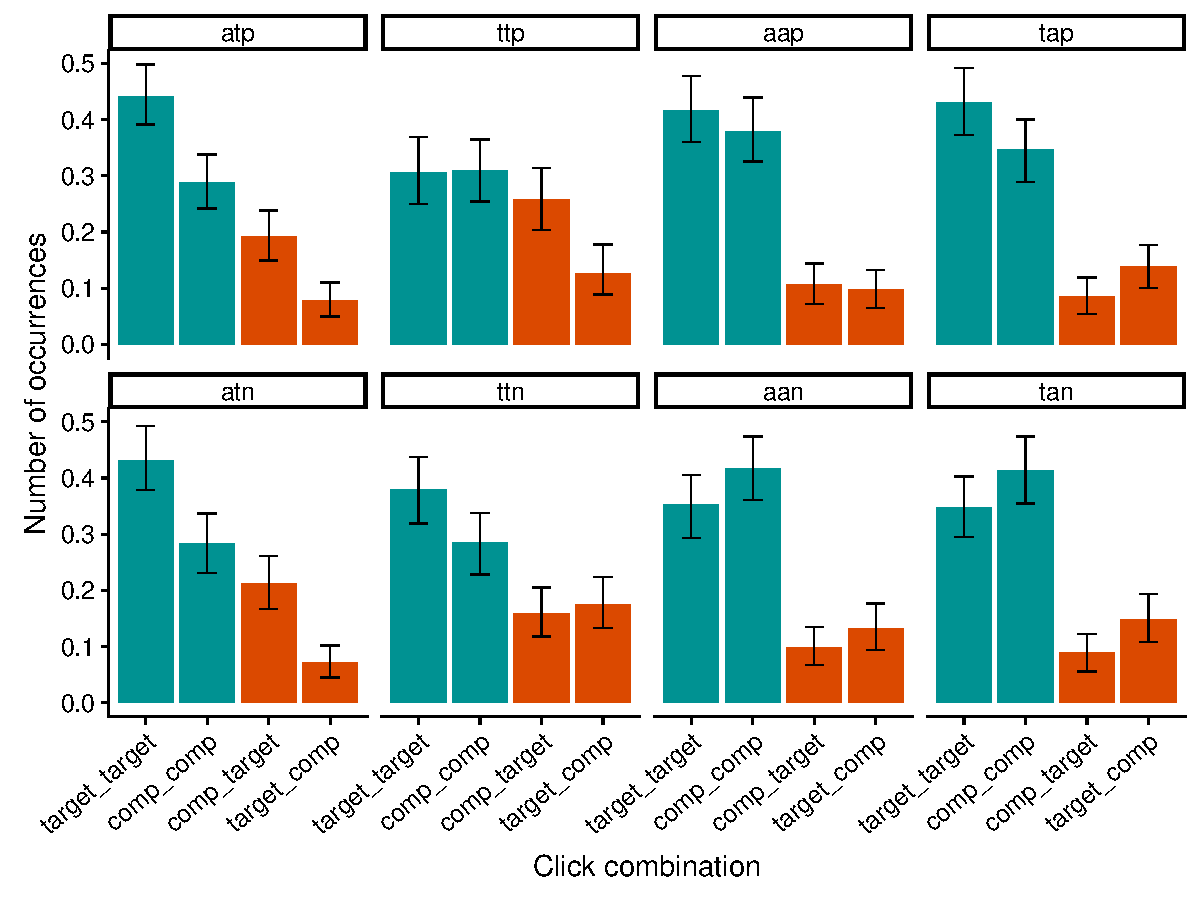
\includegraphics[width=.475\textwidth]{graphs/switching-bycond.pdf}
% 	\end{center}
% \caption{This is a figure.\ek{makes this to a collapsed plot without condition grouping? Maybe even get rid of the plot, but it makes it harder to describe.}} 
% \label{switching}
% \end{figure}

Qualitative post-hoc analyses revealed that the selections after reading the adjective were also affected by the participant's previous selection. A participant who previously selected the competitor was more likely to select the competitor again than switch to the target (and vice versa). But since the object selections before the adjective occurred are uniformly distributed, any patterns that appear after the adjective cannot be an artifact of the reselection bias.

These results clearly show that the color typicality of the objects in the display affect the inference listeners draw about the intended referent. An atypical competitor alone can promote the competitor over the target when the contrast is absent and can even make the target preference disappear when a contrast is present. It is therefore highly relevant to control for the quality of the competitor when assessing contrastive inferences. 
Choosing an atypical target makes the contrast-present and contrast-absent conditions more similar, suggesting a smaller contrastive inference. This replicates the finding that the contrastive inference did not appear with items of unpredictable colors \cite{Sedivy:2003}.

\section{Model evaluation}

To assess the relationship between the modifier production probabilities and the comprehension data in the simplest way, we will assume a flat prior over all objects in the display. This choice is further justified by the uniform distribution over all objects before receiving any information about the target in the comprehension experiment. The probabilities to choose the target over the competitor are then the normalized modifier production probabilities as shown in Equation~(\ref{eq-flatprior}), where $r$ is the possible referent, $u$ the utterance and $C$ the specific context.

\begin{equation}
	P_{L_1}(r|u,C) = \frac{P_{S_0}(u|r,C)}{P_{S_0}(u|r_{target},C) + P_{S_0}(u|r_{comp},C)}
\label{eq-flatprior}
\end{equation}

Figure~\ref{model-results-flatprior} shows the model predictions (in blue) and the empirical results (in purple) for target and competitor selection after observing the adjective. 

Using the modifier production probabilities obtained in Experiment 1, the model qualitatively predicts the patterns for the different context conditions. 

Quantitatively the RSA model is a significant predictor for the empirically elicited comprehension data ($E=1.46, CI=[1.01, 1.91]$)\footnote{Results of a Bayesian mixed effects regression model $target\_selection \sim RSA\_prediction + previous\_selection + (1+RSA\_prediction|participant)$.} and its predictions highly correlate with the empirical results ($r=0.91$). However, it generally predicts stronger inferences than borne out in the empirical data, as shown in Figure~\ref{model-results-corr-flatprior}. The model overpredicts target selection for high target preference conditions and underpredicts the target selection in low target preference conditions. 

\begin{figure}
	\begin{center}
		\includegraphics[width=.475\textwidth]{graphs/model-bycond-paper.pdf}
	\end{center}
\caption{This is a figure.} 
\label{model-results-flatprior}
\end{figure}

\begin{figure}
	\begin{center}
		\includegraphics[width=.475\textwidth]{graphs/corr-plot.pdf}
	\end{center}
\caption{This is a figure.\ek{put contrast-present up}} 
\label{model-results-corr-flatprior}
\end{figure}

One possible explanation is that the inferences appear smaller in the comprehension study, especially because of the bias to reselect the previously selected object (as described in the results of Experiment 2). If a participant receives an adjective that is supposed to elicit a contrastive inference, but the participant has clicked the competitor before, the non-switching bias will counteract the contrastive inference choice. This can explain why the preference of the target over the competitor is flatter than expected and might be an artifact of the offline incremental decision task. Since an online eye-tracking experiment does not rely on incremental selections, we expect this bias to decrease and therefore the inferences to become stronger.

% \begin{figure}
% 	\begin{center}
% 		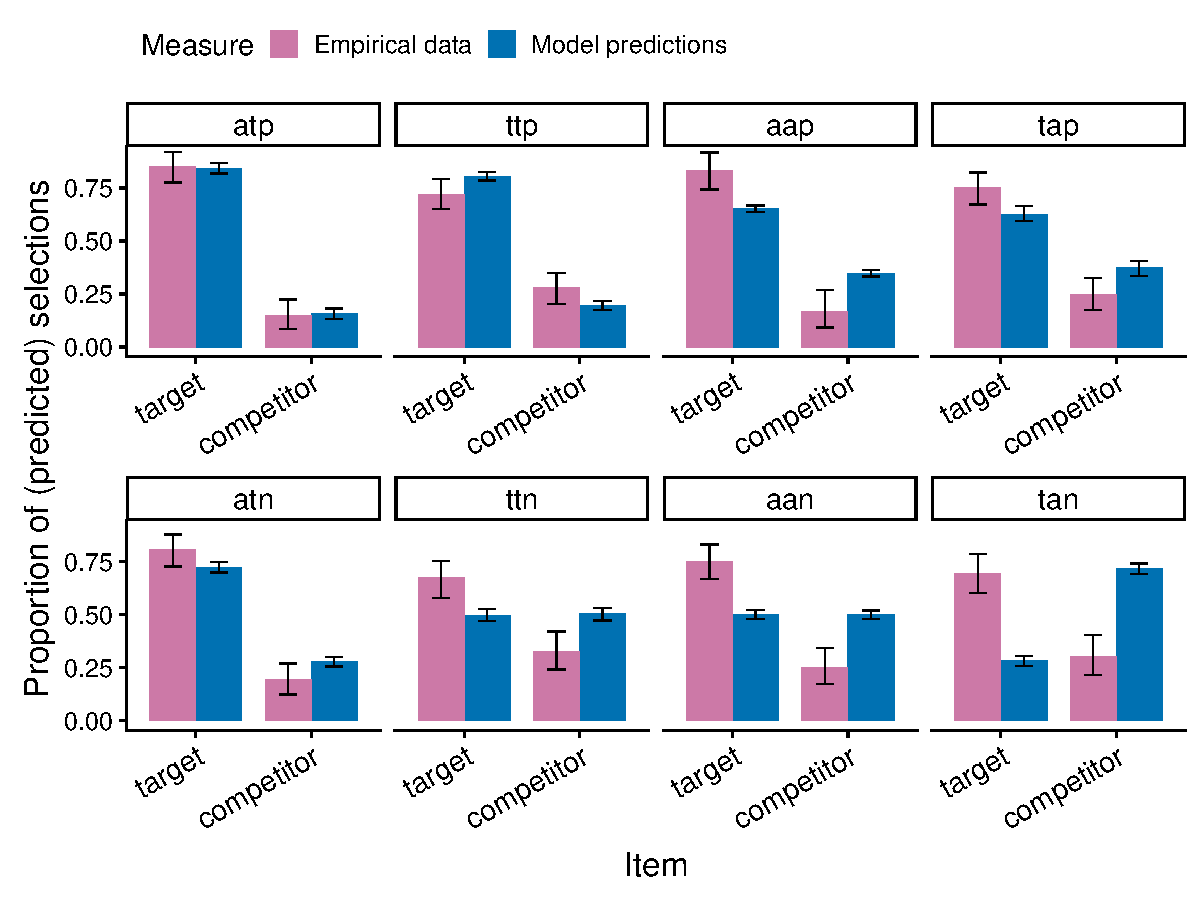
\includegraphics[width=.475\textwidth]{graphs/modelflat-bycondition-targetprevClick.pdf}
% 	\end{center}
% \caption{This is a figure.\ek{fix a lot}} 
% \label{model-results-flatprior-targetprev}
% \end{figure}

Overall, these results suggest a strong interconnection between referring expression interpretation and production. Only using the probability of encountering the utterance itself, the RSA model can qualitatively and quantitatively predict the empirically elicited comprehension data. Although we replicate that the contrastive inference can be elicited in an offline incremental decision task, the model results suggest that the selection biases in the paradigm might reduce the size of the inferences. We expect this bias to reduce in an eye-tracking paradigm, which is an immediate future direction for this work.


\section{Discussion}

In this paper, we provided a novel account of contrastive inference in which we argue for a speaker-centric model of comprehension. We use the Rational-Speech Act (RSA) framework to make quantitative predictions about the behavior a pragmatic listener \textit{should} exhibit when provided with different contexts. This account shifts the focus away from specific cognitive and linguistic factors that have been discussed to affect contrastive inference in the literature onto listener's production expectations (and their prior beliefs). We show that this speaker-centric model cannot only account for the general case of contrastive inference, but makes further predictions onto why contrastive inference appears to be less stable with color adjectives. 

In contrast to previous accounts, it is not simply the production probability of the target that matters (as suggested in a default description account \cite{Sedivy:2003}), but instead the relative modifier production probability of \emph{all} objects in the display, which are then evaluated against each other. In this particular case this means that it assigns a central role to the color competitor in the display. The empirical results confirm that the choice of the competitor affects the interpretation of the utterance, providing evidence for this highly pragmatic account of comprehension.

We assessed the model predictions by collecting object selections in an incremental decision task \cite{Qing:2018}, replicating that it generally can elicit the contrastive inference. Crucially the results show high variation between context conditions dependent on the typicality of the target and competitor. In other words, by varying the modifier production probabilities, we can make the contrastive inference appear strong and almost make it disappear. This range provides a challenge for accounts that argue for a uniform quality about adjective semantics that affect contrastive inference. A speaker-centric account predicts instead that the general differences observed between different types of adjectives is in fact mediated by how likely a listener expects the modifier to be produced and an interesting new avenue for future investigations.
















% \ek{random thought: if target is typical and contrast present -- does the typicality of the contrast affect modifier production for the target? It should. So far we see that modifier mention for the typical target + contrast contexts is not at ceiling, because (maybe) "banana" is still a better description of the target than the contrast. This would probably change if the contrast was brown.}

% You can't take the results wrt presence/size of the contrastive inference effect and draw conclusions about the nature of adjective types. We can take color adjectives and make the contrastive inference (dis-)appear, i.e., we can make them look like size or material adjectives.

% We are showing that
% 1) listeners are highly pragmatic, i.e., they consider how well the utterance fits to each possible referent in the context and draws inferences about each and then takes them together -> competitor matters
% 2) thereby the modifier does not simply seem to receive a contrastive explanation for mentioning, but also a typicality explanation which affects the final inference just as much
% 3) taken together there simply seems to be an expectation of modifier inclusion which can result from multiple rationales.
% 4) we can make the contrastive inference strong (as for size adjectives) or disappear
% 5) in RSA we don't need to assume anything about the nature of the adjective, but can simply consider what the speaker probabilities for modifier use are... i.e., the linguistic knowledge can be obscure: we just need to consider production probabilities to predict listener behavior; underlyingly this could be simply communicative pressures; Due to informativity, the color needs to be mentioned if there is a contrast and the same holds for typicality (see PsychReview paper)

% \ek{thought: the term contrastive inference is so confusing. Because there is a contrastive inference in the tan-tap case, but it's not simply: "Is there a target preference in the contrast present case", but is there a target preference compared to the non-contrast condition. I.e., if you define the contrastive inference as the preference of the target over the competitor when the contrast is present, there is no contrastive inference in the tap condition. But if you define it as the change in preference from contrast absent to contrast present, then there still is a contrastive inference. This issue makes describing the "occurrence of contrastive inference" difficult here -- maybe we should address that?}




























% \section{General Formatting Instructions}

% The entire content of a paper (including figures, references, and anything else) can be no longer than six pages in the \textbf{initial submission}. In the \textbf{final submission}, the text of the paper, including an author line, must fit on six pages. Up to one additional page can be used for acknowledgements and references.

% The text of the paper should be formatted in two columns with an
% overall width of 7 inches (17.8 cm) and length of 9.25 inches (23.5
% cm), with 0.25 inches between the columns. Leave two line spaces
% between the last author listed and the text of the paper; the text of
% the paper (starting with the abstract) should begin no less than 2.75 inches below the top of the
% page. The left margin should be 0.75 inches and the top margin should
% be 1 inch.  \textbf{The right and bottom margins will depend on
%   whether you use U.S. letter or A4 paper, so you must be sure to
%   measure the width of the printed text.} Use 10~point Times Roman
% with 12~point vertical spacing, unless otherwise specified.

% The title should be in 14~point bold font, centered. The title should
% be formatted with initial caps (the first letter of content words
% capitalized and the rest lower case). In the initial submission, the
% phrase ``Anonymous CogSci submission'' should appear below the title,
% centered, in 11~point bold font.  In the final submission, each
% author's name should appear on a separate line, 11~point bold, and
% centered, with the author's email address in parentheses. Under each
% author's name list the author's affiliation and postal address in
% ordinary 10~point type.

% Indent the first line of each paragraph by 1/8~inch (except for the
% first paragraph of a new section). Do not add extra vertical space
% between paragraphs.


% \section{First Level Headings}

% First level headings should be in 12~point, initial caps, bold and
% centered. Leave one line space above the heading and 1/4~line space
% below the heading.


% \subsection{Second Level Headings}

% Second level headings should be 11~point, initial caps, bold, and
% flush left. Leave one line space above the heading and 1/4~line
% space below the heading.


% \subsubsection{Third Level Headings}

% Third level headings should be 10~point, initial caps, bold, and flush
% left. Leave one line space above the heading, but no space after the
% heading.


% \section{Formalities, Footnotes, and Floats}

% Use standard APA citation format. Citations within the text should
% include the author's last name and year. If the authors' names are
% included in the sentence, place only the year in parentheses, as in
% \citeA{NewellSimon1972a}, but otherwise place the entire reference in
% parentheses with the authors and year separated by a comma
% \cite{NewellSimon1972a}. List multiple references alphabetically and
% separate them by semicolons
% \cite{ChalnickBillman1988a,NewellSimon1972a}. Use the
% ``et~al.'' construction only after listing all the authors to a
% publication in an earlier reference and for citations with four or
% more authors.


% \subsection{Footnotes}

% Indicate footnotes with a number\footnote{Sample of the first
% footnote.} in the text. Place the footnotes in 9~point font at the
% bottom of the column on which they appear. Precede the footnote block
% with a horizontal rule.\footnote{Sample of the second footnote.}


% \subsection{Tables}

% Number tables consecutively. Place the table number and title (in
% 10~point) above the table with one line space above the caption and
% one line space below it, as in Table~\ref{sample-table}. You may float
% tables to the top or bottom of a column, and you may set wide tables across
% both columns.

% \begin{table}[H]
% \begin{center} 
% \caption{Sample table title.} 
% \label{sample-table} 
% \vskip 0.12in
% \begin{tabular}{ll} 
% \hline
% Error type    &  Example \\
% \hline
% Take smaller        &   63 - 44 = 21 \\
% Always borrow~~~~   &   96 - 42 = 34 \\
% 0 - N = N           &   70 - 47 = 37 \\
% 0 - N = 0           &   70 - 47 = 30 \\
% \hline
% \end{tabular} 
% \end{center} 
% \end{table}


% \subsection{Figures}

% All artwork must be very dark for purposes of reproduction and should
% not be hand drawn. Number figures sequentially, placing the figure
% number and caption, in 10~point, after the figure with one line space
% above the caption and one line space below it, as in
% Figure~\ref{sample-figure}. If necessary, leave extra white space at
% the bottom of the page to avoid splitting the figure and figure
% caption. You may float figures to the top or bottom of a column, and
% you may set wide figures across both columns.

% \begin{figure}[H]
% \begin{center}
% \fbox{CoGNiTiVe ScIeNcE}
% \end{center}
% \caption{This is a figure.} 
% \label{sample-figure}
% \end{figure}


% \section{Acknowledgments}

% In the \textbf{initial submission}, please \textbf{do not include
%   acknowledgements}, to preserve anonymity.  In the \textbf{final submission},
% place acknowledgments (including funding information) in a section \textbf{at
% the end of the paper}.


% \section{References Instructions}

% Follow the APA Publication Manual for citation format, both within the
% text and in the reference list, with the following exceptions: (a) do
% not cite the page numbers of any book, including chapters in edited
% volumes; (b) use the same format for unpublished references as for
% published ones. Alphabetize references by the surnames of the authors,
% with single author entries preceding multiple author entries. Order
% references by the same authors by the year of publication, with the
% earliest first.

% Use a first level section heading, ``{\bf References}'', as shown
% below. Use a hanging indent style, with the first line of the
% reference flush against the left margin and subsequent lines indented
% by 1/8~inch. Below are example references for a conference paper, book
% chapter, journal article, dissertation, book, technical report, and
% edited volume, respectively.

% \nocite{ChalnickBillman1988a}
% \nocite{Feigenbaum1963a}
% \nocite{Hill1983a}
% \nocite{OhlssonLangley1985a}
% % \nocite{Lewis1978a}
% \nocite{Matlock2001}
% \nocite{NewellSimon1972a}
% \nocite{ShragerLangley1990a}


\bibliographystyle{apacite}

\setlength{\bibleftmargin}{.125in}
\setlength{\bibindent}{-\bibleftmargin}

\bibliography{CogSci_Template}


\end{document}
